\documentclass[12pt,twoside,english,french]
\author{Bertrand Guerrero}
\usepackage{etex}
\usepackage{lmodern}
\renewcommand{\familydefault}{\rmdefault}
\usepackage[T1]{fontenc}
\usepackage[utf8x]{inputenc}
\usepackage[a4paper]{geometry}
\geometry{verbose,tmargin=3.5cm,bmargin=3cm,lmargin=3cm,rmargin=2cm,headsep=1.75cm}
%\setcounter{secnumdepth}{4}
%\setcounter{tocdepth}{4}
\usepackage[francais]{babel}
\addto\extrasfrench{%
   \providecommand{\og}{\leavevmode\flqq~}%
   \providecommand{\fg}{\ifdim\lastskip>\z@\unskip\fi~\frqq}%
}
\usepackage[thinlines]{easymat}
\usepackage{lscape}
\usepackage{pslatex}
\usepackage{txfonts}
\usepackage{footnote}
%\usepackage{mathptmx}
\usepackage{setspace}
\usepackage{natbib}
\onehalfspacing
\usepackage[unicode=true,
 bookmarks=true,bookmarksnumbered=false,bookmarksopen=false,
 breaklinks=true,pdfborder={0 0 0},backref=false,colorlinks=true, citecolor=Gray, linkcolor=blue, urlcolor=blue]
 {hyperref}
%\usepackage{numprint}
\usepackage{breakurl}
\usepackage{graphics}
\usepackage{graphicx}
\usepackage{natbib}
\usepackage{here}
\usepackage{float}
\usepackage[french, ruled, vlined]{algorithm2e}
\graphicspath{{Images/}}
\usepackage{caption}
\usepackage{subcaption}
\captionsetup{figurewithin=none}  
\captionsetup{tablewithin=none}
\usepackage{lettrine}
\renewcommand{\LettrineFontHook}{\color[gray]{0.5}}
\usepackage[svgnames]{xcolor}
\xdefinecolor{DarkOliveGreen}{named}{DarkOliveGreen}
\usepackage{multirow}
\usepackage{float}
\usepackage{wrapfig}
\usepackage[]{tocbibind}
\usepackage{makeidx}
\usepackage{textcomp}
\usepackage[final]{pdfpages} 





\makeatletter



\makeindex
\newenvironment{changemargin}[2]{\begin{list}{}{%
\setlength{\topsep}{0pt}%
\setlength{\leftmargin}{0pt}%
\setlength{\rightmargin}{0pt}%
\setlength{\listparindent}{\parindent}%
\setlength{\itemindent}{\parindent}%
\setlength{\parsep}{0pt plus 1pt}%
\addtolength{\leftmargin}{#1}%
\addtolength{\rightmargin}{#2}%
}\item }{\end{list}}

%%%%%%%%%%%%%%%%%%%%%%%%%%%%%% LyX specific LaTeX commands.
%% Because html converters don't know tabularnewline
\providecommand{\tabularnewline}{\\}

%%%%%%%%%%%%%%%%%%%%%%%%%%%%%% Textclass specific LaTeX commands.
\usepackage{enumitem}		% customizable list environments
\newlength{\lyxlabelwidth}      % auxiliary length 

%%%%%%%%%%%%%%%%%%%%%%%%%%%%%% User specified LaTeX commands.
\renewcommand{\thefigure}{\ifnum \c@chapter>\z@ \thechapter.\fi
 \@arabic\c@figure}
\@addtoreset{figure}{chapter}

\renewcommand{\thetable}{\ifnum \c@chapter>\z@ \thechapter.\fi
 \@arabic\c@table}
\@addtoreset{table}{chapter}



\makeatother

\begin{document}

%\paragraph*{\pagenumbering{Roman}}

\includepdf{page_garde.pdf}

\pagenumbering{roman} \setcounter{page}{1} 

\chapter*{Remerciements}
%\tableofcontents


Je tiens tout d’abord à remercier mon maître de stage Christophe Lapierre qui m’a permis de réaliser mon stage dans les meilleures conditions possibles. 
Je le remercie pour ses conseils, le temps qu’il m’a consacré et pour ses commentaires sur mon travail. \\

Je remercie Julien Lesbegueries pour m'avoir intégré dans son projet, m'avoir permis au cours du stage de découvrir des technologies telles que Dropwizard et pour toutes les bonnes pratiques de développement qu'il m'a transmises.\\

Merci à mes deux « super » formateurs Gilles Vanderstraeten (Java SE) et Laure Bouquety (Java EE), pour leurs cours et leur support, ils m'ont appris et fait aimer le langage Java. \\

Merci à Florian pour les pauses, et à Wafi pour ses dessins de réseaux sur mon bureau.\\

Enfin, je voudrais remercier particulièrement Frédéric Schettini de m’avoir donner cette opportunité de stage qui rentre pleinement dans mon projet professionnel, tant par les aspects techniques que par leurs domaines d'application. \\


\chapter*{Abstract}


My internship subject focuses on developing web services that expose the functionality of road and transit data import, for automatic build of multi-modal transport networks. \\

The objective of my work is to expose functionality originally coded in SQL and / or Python via a REST API (JAX-RS). So I initially took over the treatment of warps (ArcPy / Python) and learned to manipulate the data (PostGIS / GTFS) via the project "DataWizard". In parallel, in order to implement these REST web services (Java EE) I joined the project "MobiSaaS" and discovered to develop with the "DropWizard" framework oriented micro-services. \\

The application developed in the project "MobiSaaS" has an administration interface to expose features of MobiAnalyst package \footnote{\url{http://www.mobianalyst.fr/}} like a SaaS. It is in this context that I develop features data upload to the server. So, I realized all my development in a Maven module included in an existing mutli-modules project. My development was carried out mode "concurrency" to support multiple concurrent requests, and make the asynchronous service. Finally as prospects, classes and utilities methods I developed will be generalized so that the "Upload" service supports several other data formats (vector data "Shapefile" for example). \\

During this internship I worked on several projects: DataWizard, Crislab, MobiSaaS, etc ... So I participated in various phases of of software development lifecycle (from design ( R \ & D), development of business code, until delivery to the customer). \\

 

\renewcommand{\contentsname}{Sommaire} %dans le corps du document, avant la commande \tableofcontents .

\tableofcontents

\pagenumbering{arabic} \setcounter{page}{1} 

\chapter{Introduction} 
\label{Introduction}

Ce stage s'inscrit dans le cadre de la formation "Concepteur / Développeur Informatique" délivrée par BGE Haute-Garonne et s'est déroulé durant 3 mois au sein de l'entreprise Mobigis. Les objectifs à l'issue de cette formation sont de savoir concevoir et développer des applications informatiques en utilisant le langage Java/JavaEE, dans un environnement professionnel.\\

Dans ce mémoire sera présenté le travail que j'ai réalisé, avec par exemple les résultats directs de mon action. Mais aussi, les tâches que j'ai effectuées et les moyens utilisés pour les accomplir : langages, frameworks, logiciels,…\\
 
Cette présentation s'organise de la façon suivante:\newline

\begin{itemize}
\item Une première partie sera dédiée à la présentation du contexte du stage. Dans cette partie seront présentés le domaine d'application de ce stage : les Systèmes d'Informations Géographiques (SIG), et l'entreprise MobiGIS.\\

\item Dans la deuxième partie, l'environnement de travail du stage sera expliqué : projets, équipes, outils, produits,...\\

\item Une troisième partie présentera la méthodologie de mon travail (conception/développement) et des exemples de réalisations (codes)...\\

\item Enfin, dans la dernière partie de ce mémoire seront présentés un bilan professionnel et un bilan personnel de cette nouvelle expérience.\newline

\end{itemize}

Par la suite, les termes en \textbf{gras} seront définis dans le glossaire en fin du mémoire.



\chapter{Contexte du stage}
\label{AnalyseConception}

\section{Environnement de travail}

Durant le stage j'ai travaillé sur un pc dont le système d'exploitation est Windows 8.1 Profesionnal (machine hôte). L'entreprise travaille avec de nombreuses machines virtuelles hébergées ou distantes afin de disposer d'environnement de tests, de développements, et de production. J'avais donc à ma disposition une machine virtuelle de développement via VirtualBox dont le système d'exploitation était Windows Server 2012 R2 Standard. 
J'ai eu la chance d'arriver et de \og trouver \fg une machine pré-configurée avec tous les outils nécessaires pour développer, (le clone de cette machine virtuelle de développement a servi à d'autres stagiaires), ainsi l'administrateur système de MobiGIS maîtrise la configuration logicielle des machines.\\

\section{Outils utilisés}

Quotidiennement j'ai utilisé 2 environnements de développement intégré (IDE) : Liclipse (pour développer en langage Python) dans le projet DataWizard, et \textbf{Eclipse} version Mars (pour développer en langage Java/Java EE) pour les projets MobiSAAS et Crislab.\\

Dans les projets plusieurs \textbf{SGBD} sont manipulés : MongoDB (MobiSAAS), Oracle (Crislab), mais j'ai principalement travaillé avec \textbf{Postgresql} afin de gérer les données de mon module. De plus, Postgresql permet de gérer les données géographiques dans le projet \og DataWizard \fg grâce à sa cartouche spatiale \textbf{Postgis}.\\

Les logiciels suivants ont été utilisés quotidiennement : Maven, DropWizard, Hibernate, Jackson, Postgresql, Pgadmin, \textbf{SoapUI}, Java JDK 1.7 et 1.8. Certains de ces outils seront décrits dans la suite de ce mémoire \ref{MobiSAASTechno}.
J'ai également essayé de produire des schémas pour la documentation avec des logiciels de « modélisation » comme : ArgoUML, DBVisualizer, Enterprise Architect, yEd.\\

\section{Gestion de projets}

Dans les projets auxquels j'ai participé, l'entreprise utilise des outils de gestion : planning, suivi de bugs, outils de mutualisation, gestion de versions. Ainsi, j'ai utilisé l'outil Trello pour la gestion des tâches, Redmine pour la gestion des projets (cf. Annexe \ref{Annexe A}), et \textbf{SVN} pour la gestion des codes sources. L'entreprise met à disposition de ses salariés un intranet avec de nombreux outils collaboratifs sous la plateforme eGroupware (feuille de temps,etc...).\\

J'ai effectué mon travail en étroite relation avec le chef de projet. A partir des spécifications techniques et fonctionnelles, les développements ont progressé et évolué tout le long de la période de réalisation. Sans pour autant pratiquer une méthode «Agile» au sens strict, plusieurs ajustements (mode itératif) ont été effectués et le dialogue quotidien à permis de toujours rendre mon travail en adéquation aux besoins. \\

Un point de suivi informel était effectué plusieurs fois par semaine avec mon responsable afin de présenter le travail effectué, les résultats intermédiaires, et le travail planifié pour la semaine suivante. Un bilan à la mi-stage a été effectué afin de réajuster les priorités, et arriver à produire un livrable satisfaisant en fin de stage. \\


\section{Difficultés rencontrées}

Il y a peu à dire, l'environnement "équipe" et les compétences de chacun ont été propices à les éviter. En effet, j'avais de chaque côté de mon bureau les 2 personnes les plus à même de débloquer des situations, ou de me renseigner sur une question. \\

Pour le projet MobiSAAS, j'ai eu des "difficultés" qui sont communes à chaque évolution de version d'un \textbf{framework}. En effet, au milieu du stage il a fallu "recoder" dans plusieurs parties du code pour s'adapter aux évolutions lors du passage de la version 0.7.1 à la version 0.8.1 de Dropwizard.
Sinon, pour le projet DataWizard et d'une manière générale, une des difficulté a été de répondre aux experts et analystes en réseaux de transport et produire des résultats (Métadonnées) exploitables et conformes à leurs attentes. Cela a demandé du dialogue et de se mettre en accord sur la terminologie à employer (ex: EdgeType, PTMode,...). Tous ces termes courants pour les experts ne sont pas intuitifs pour les développeurs... Encore une fois, je pense que cette \og difficulté \fg liée à un aspect métier est commun à tous les projets.\\


\chapter{Les Projets}
\label{Developpement}

\section{MobiSAAS}

\subsection{Cahier des charges, présentation de l'application}

Le projet \og MobiSAAS \fg : MobiAnalyst as a Service, s'inscrit dans la démarche d'entreprise de proposer des solutions en mode \textbf{SAAS}. Le projet consiste d'une manière générale à exposer les fonctionnalités de la solution Desktop du produit \og MobiAnalyst\footnote{\url{http://www.mobianalyst.fr/}} \fg. C'est pour ce projet que j'ai effectué mon travail de stage. \\

\begin{figure}[!h]
\centering
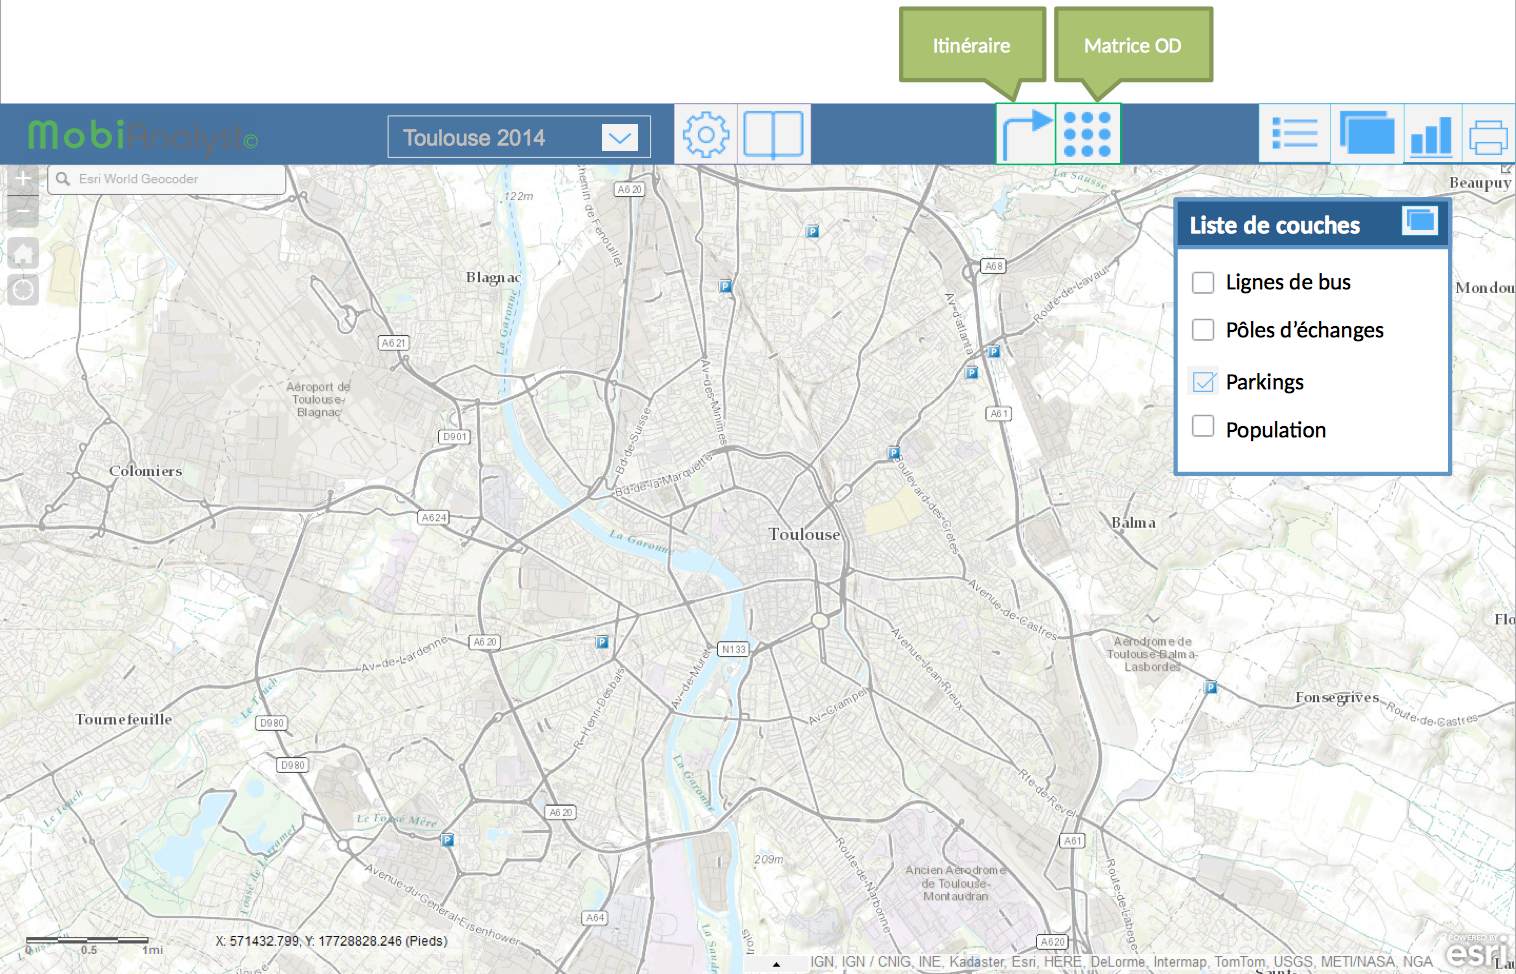
\includegraphics[width=16cm]{images/MobiSAAS_IHM.png}
\caption{\label{MobiSAAS_IHM.png}Interface de MobiSAAS (frontend)}
\end{figure} 
\\


Mon sujet de stage porte sur le développement de \textbf{web services} permettant d'exposer des fonctionnalités d'importation de données voirie et transport en commun, pour la construction automatique de réseaux de transports multi-modaux (graphes)(Fig. \ref{OffreMobiAnalyst}). \\

\begin{figure}[h]
\centering
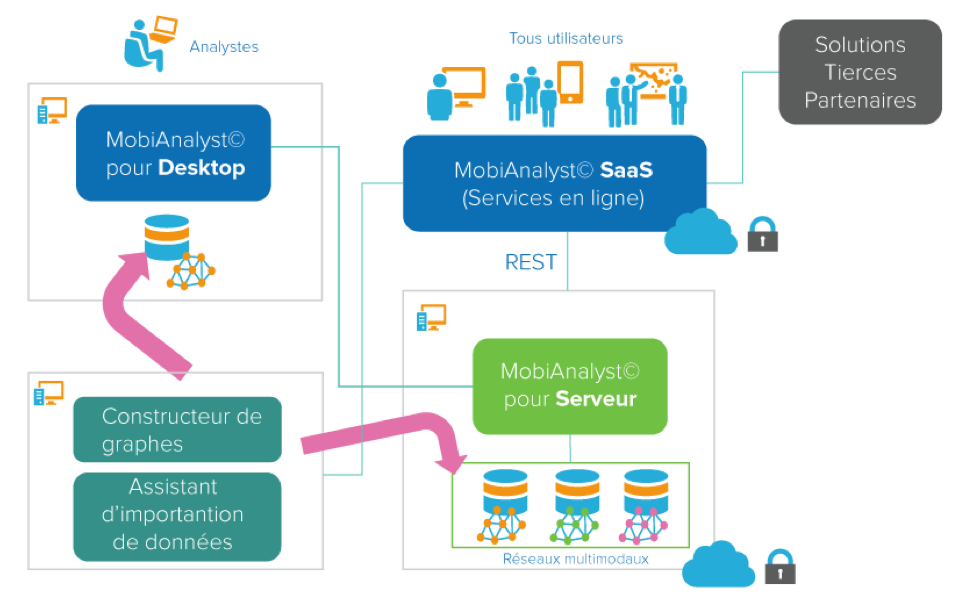
\includegraphics[width=16cm]{images/offre_MobiAnalyst.png}
\caption{\label{OffreMobiAnalyst}Offres du produit MobiAnalyst}
\end{figure} 
\\

Les serveurs MobiAnalyst propose une \textbf{API} de services web de type \textbf{REST} avec des fonctions bas niveau :
\begin{itemize}
\item Calcul d'un itinéraire multi-modal 
\item Calcul d'un isochrone multi-modal
\item Calcul d'une MOD
\item Géotraitements d'analyse réseaux 
\end{itemize}

C'est dans le cadre de l'interface d'administration de l'application (backend) que je devais développer des fonctionnalités d'upload de données de transport (GTFS\footnote{\url{https://developers.google.com/transit/gtfs/}}) sur le serveur.\\

L'objectif de mon travail a été d'exposer des fonctionnalités (en vert sur Fig. \ref{OffreMobiAnalyst}) codées initialement en langage SQL et/ou Python via une API REST en langage Java (JAX-RS). 

J'ai donc dans un premier temps pris en main les chaînes de traitements (Python) et appris à manipuler les données (Postgis/SQL) via le projet \og DataWizard \fg. En parallèle, afin d'implémenter ces web services j'ai intégré le projet « MobiSAAS » et ainsi appris à développer avec le framework \og Dropwizard \fg. \\

\paragraph{Une API REST ?}\\

Pour commencer ce travail, j'ai déjà découvert ce qu'est une API REST et surtout comment la designer (maquetter). Je me suis inspiré du très bon article suivant \url{http://blog.octo.com/designer-une-api-rest/ } dont voici les grands principes à retenir :

\item REST est un style d'architecture orienté ressource (ROA).
\item L'abstraction clé de l'information en REST est une « Ressource ». N'importe quelle information qui peut être nommée est une ressource : une image, un document, un service temporel (la météo d'aujourd'hui à Toulouse), une collection d'autres ressources, un objet physique (une personne) etc. En d'autres termes, n'importe quel concept qui peut être la cible d'une référence d'un lien hypertexte doit s'adapter dans la notion de ressource.
\item L'API doit donc proposer des web services sur ces ressources qui répondent aux requêtes du protocole HTTP. (cf. Tableau).
\item Le concept de représentation (XML/JSON) est important. Nous avons choisi de ne représenter les résultats de requêtes (Response) que via le format d'échange de données JSON (JavaScript Object Notation).
\item Une dernier concept fondamental sont les réponses de ces services. Le WS peut renvoyer soit des données (JSON), et des codes HTTP (cf. Tableau). Il est préconisé d'utiliser les codes de retour HTTP (500, 404, 200), de manière appropriée, sachant qu'il existe un code pour chaque cas d'utilisation courant. Ces codes sont connus de tous. Pour les besoins de l'API nous avons spécifié des codes propres à l'application et au contexte (601, 602, 603) (cf. Tableau).


\subsubsection{Architecture actuelle}

La figure \ref{fig:architectureMobiAdmin} détaille l'ensemble des briques logicielles nécessaires au fonctionnement de la plate-forme MobiSAAS :
\begin{itemize}
\item \textbf{AGS} : ArcGIS Server. Le serveur de Système d'Information Géographique (SIG) permettant de publier et d'administrer des services cartographiques (MapService).
Dans notre cas, les MapServices déployés sont des réseaux routiers et de transport en commun (TC), accompagnés de tables horaires (TimeTable) contenant les horaires des TC.
\item \textbf{SOE}: Server Object Extension. Nous utilisons le mécanisme d'extension \og SOE \fg pour déployer sur un MapService un service spécifique à MobiSAAS. Un SOE est une fonctionnalité qui se déploie sur un MapService et qui expose en Web Service (REST ou SOAP) les solveurs (algorithme de résolution d'itinéraires) de MobiAnalyst.
\item \textbf{MobiAdmin}: Serveur REST d'administration MobiSAAS. Ce serveur (basé sur Java) est le point d'entrée des utilisateurs des services REST de MobiAnalyst.
Il redirige les requêtes métiers vers le bon SOE déployé, il trace ces requêtes et enrichit la base de données client de MobiAnalyst.
L'authentification qui est faite dans les requêtes utilise les comptes d'AGS créés au préalable.
\item \textbf{Postgres} : Système de gestion de base de données. Cette base contient les données clients de MobiAnalyst : profil, traces d'utilisation de MobiSAAS.
\item \textbf{MongoDB} : Système de gestion de base de données. Cette base contient les logs (statistiques mesurées en temps réel) correspondant aux services REST de MobiSAAS.
\end{itemize}\\

\begin{figure}[!h]
	\centering
		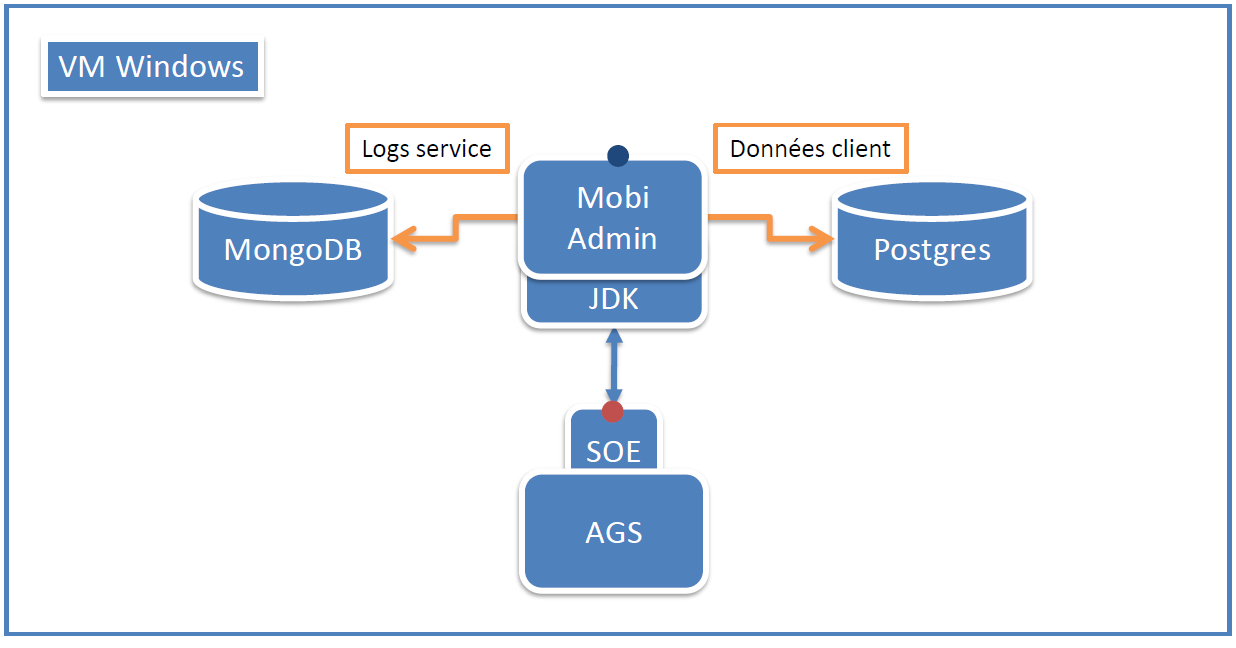
\includegraphics[width=0.8\textwidth]{images/architecture.png}
	\caption{Architecture globale de \og MobiAdmin \fg}
	\label{fig:architectureMobiAdmin}
\end{figure}\\

\subsection{Eléments de spécifications fonctionnelles}

Mon stage et les développements demandés concernent le composant d'administration de l'infrastructure : \og MobiAdmin \fg (cf. Fig. \ref{fig:architectureMobiAdmin}). Dans l'objectif de gérer les données du client, je dois proposer un web service pour la gestion des données de transport dans l'espace privatif du client.
La fonctionnalité principale à développer est donc un web service d'upload de données et plus particulièrement l'upload de données de transport public au format GTFS\footnote{\url{https://developers.google.com/transit/gtfs/reference}}.\\ 

Les données GTFS se présente le plus souvent dans une archive contenant au minimum les 8 fichiers .txt suivants :
\\
\begin{figure}[h]
	\centering
		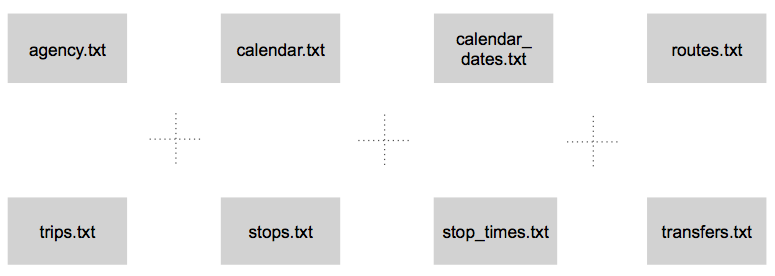
\includegraphics[width=0.8\textwidth]{images/GTFS_8fichiers.png}
	\caption{Contenu des données GTFS}
	\label{fig:GTFS_8fichiers}
\end{figure}\\


L'objectif de ce service d'import de données GTFS est de à plus termes pouvoir manipuler ces données (fichier au format zip), pouvoir récupérer des métadonnées sur les jeux de données exemple : l'extension géographique des données, le nom de l'agence, le nombre de lignes, le mode de transport, et enfin produire un réseau de transport via un service en ligne. Actuellement, ces fonctionnalités sont réalisées en amont du logiciel MobiAnalyst via le logiciel Desktop DataWizard (cf. \ref{DataWizard} DataWizard).\\

Une archive ou  \og Upload \fg de données GTFS peut contenir un seul ou plusieurs jeu de données (ensemble de fichiers .txt). Il faut donc récupérer et renseigner les métadonnées de chaque Upload sur le serveur :
\begin{itemize}
\item Nom - UUID (identifiant unique)
\item Date d'upload
\item Status d'upload (SUCCESS, FAILED, LOADING, INIT)
\item Nom de l'archive (source)
\item Chemin vers le rapport de validation GTFS
\item Chemin vers la données

\end{itemsize}\\

Les résultats attendus sont le stockage sur le serveur (système de fichier) des données envoyées par le client, stocker la trace de l'opération dans un SGBD, et enfin la production de réponses HTTP (format JSON) pour chaque requête sur le service.\\

Ce service dédié aux données GTFS est très spécifique. Une attention particulière sera faite afin de développer de manière à abstraire et rendre au maximum générique la plupart des composants afin de proposer d'autres format de données à l'importation sur le serveur REST \og MobiAdmin \fg (utilisation d'interfaces et de classes abstraites).\\

\subsection{Eléments de spécifications techniques}

Pour le composant \og MobiAdmin \fg (serveur REST) qui va héberger les services, le choix technologique majeur est d'utiliser le framework DropWizard (cf. \ref{Dropwizard}). Ce framework orienté microservices nous permet de fournir notamment un serveur embarqué HTTP \og Jetty \fg. Et le framework open source Jersey pour la partie webservice REST qui est l'implémentation de référence de la spécification JAX-RS. Ou encore la librairie Jackson \og King of JSON \fg pour la sérialisation/désérialisation du JSON.\\

L'environnement de développement est donc un projet Java EE Maven (cf. \ref{Maven}) composé des éléments de Dropwizard. 
Les \textbf{WS} exposés sont à priori \og lourds \fg, sachant qu'un jeu de données peut faire jusqu'à plusieurs centaines de Mo, les opérations de téléchargement, validation, traitement, stockage dans en base,... vont être long à renvoyer une réponse au client après chaque requête. Les WS à développer sont donc asynchrones. De plus, une contrainte supplémentaire est que le service doit supporter plusieurs requêtes simultanées, il faudra donc s'orienter vers un développement en mode \og programmation concurrente \fg.\\

\subsubsection{Technologies utilisées}\label{MobiSAASTechno}

\textbf{Apache Maven : } \label{Maven}

\begin{wrapfigure}{l}{3cm}
\centering

\includegraphics[width=3cm]{images/apacheMaven.jpg}
\end{wrapfigure}
\noindent C'est un outil pour la gestion et l'automatisation de production des projets logiciels Java en général et Java EE en particulier. L'objectif recherché est comparable au système Make sous Unix : produire un logiciel à partir de ses sources, en optimisant les tâches réalisées à cette fin et en garantissant le bon ordre de fabrication.\\
Il est semblable à l'outil Ant, mais fournit des moyens de configuration plus simples, eux aussi basés sur le format XML. Maven est géré par l'organisation Apache Software Foundation. Précédemment Maven était une branche de l'organisation Jakarta Project.\\
Maven utilise un paradigme connu sous le nom de Project Object Model (POM) afin de décrire un projet logiciel, ses dépendances avec des modules externes et l'ordre à suivre pour sa production. Il est livré avec un grand nombre de tâches pré-définies, comme la compilation de code Java ou encore sa modularisation.\\
Un élément clé et relativement spécifique de Maven est son aptitude à fonctionner en réseau. Une des motivations historiques de cet outil est de fournir un moyen de synchroniser des projets indépendants : publication standardisée d'information, distribution automatique de modules « jar ». Ainsi en version de base, Maven peut dynamiquement télécharger du matériel sur des dépôts logiciels connus. Il propose ainsi la synchronisation transparente de modules nécessaires.\\

Dans le projet MobiSAAS, Maven est très utilisé car c'est un projet multi-modules avec un module parent. Maven me permet donc de télécharger et de gérer les dépendances du projet. Par exemple, voici une extrait du fichier \textbf{POM} du module utilitaire \og mobi-admin-util \fg que j'ai développé (Fig. \ref{fig:MavenPOM}).\\

\begin{figure}[!h]
	\centering
		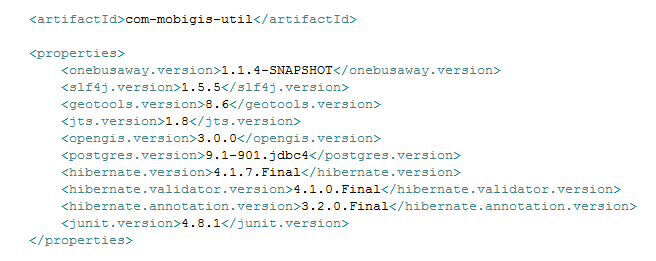
\includegraphics[width=0.8\textwidth]{images/Maven_POM_properties_Mobi-Admin-util.PNG}
	\caption{\label{fig:MavenPOM}Extrait du fichier POM, versions des dépendances utilisées}
\end{figure}
\\

\textbf{Dropwizard :}\label{Dropwizard}

\begin{wrapfigure}{l}{3cm}
\centering

\includegraphics[width=3cm]{images/dropwizard.png}
\end{wrapfigure}
\noindent C'est un framework Java léger adapté au développement rapide de microservices REST et ne nécessitant pas de serveur d'application comme environnement d'exécution.
Cela dit, au delà du framework, c'est surtout un assemblage habile de composants spécialisés parmi les meilleurs de l'écosystème Java :\\
\begin{itemize}
\item \textbf{Jetty}, un serveur HTTP et un moteur de servlet
\item \textbf{Jersey}, l'implémentation de référence de la spécification JAX-RS (web services REST) 
\item \textbf{Jackson}, une librairie de sérialisation/dé-sérialisation JSON 
\item \textbf{Hibernate Validator}, l'implémentation de référence de l'API Bean Validation (JSR 303) 
\item \textbf{SLF4J} et \textbf{Logback} pour la gestion des traces 
\item \textbf{Metrics} pour le monitoring 
\item \textbf{jDBI} pour l'interfaçage rapide à une base de données relationnelle. Cette librairie est de bien plus bas niveau que JPA ou Hibernate et présente peu d'abstraction ce qui rend sa prise en main aisée \\
\end{itemize}

Packagée sous la forme d'un jar autonome contenant toutes ses dépendances, l'unité de déploiement n'a pas besoin de serveur d'application pour être exécutée (le conteneur Jetty est embarqué dans le jar). Avec ses 10 Mo tout au plus (dépendances comprises) l'empreinte mémoire d'une application Dropwizard est donc incomparablement plus faible qu'un Web Service SOAP déployé dans un serveur d'application Java EE (jusqu'à plusieurs centaines de Mo).
En conséquences, le temps de démarrage d'une application Dropwizard est de quelques secondes quand il faut parfois plusieurs minutes pour un serveur d'application.\\

On peut considérer ce projet comme une alternative crédible aux serveurs d'applications Java EE perçus comme lourds, compliqués et gourmands en ressources. Le champ des applications couvert par Dropwizard est en réalité plus vaste que celui des microservices (il est tout a fait possible de développer une IHM web) mais l'aisance avec laquelle on développe et déploie un service REST en fait une solution très adaptée à ce type d'usage (à l'instar de Spring Boot de Pivotal ou Spark avec lesquels il est en compétition).\\

La structure d'une application Dropwizard de type API RESTful selon les préconisations d'organisation de projet du framework Dropwizard  (cf. Fig ~\ref{Organisation_Dropwizard}) est : 
\\
\begin{figure}[h]
\centering
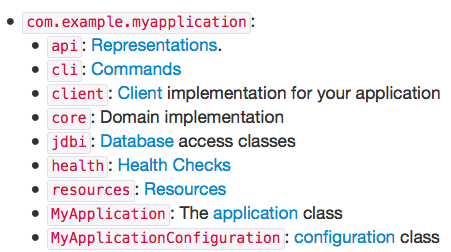
\includegraphics[width=6cm,heigth=6cm]{images/Dropwizard_Project.png}
\caption{\label{Organisation_Dropwizard}Organisation conseillée d'un projet Dropwizard}
\end{figure} 

A partir de cette organisation, nous avons structuré le module \og MobiAdmin \fg comme le montre la figure ci-dessous (cf. Fig ~\ref{Organisation_MobiAdmin}). 
Plusieurs packages spécifiques ou de configuration supplémentaires apparaissent (auth, dao, jsonable, thread,...). 
\\
\begin{figure}[h]
\centering
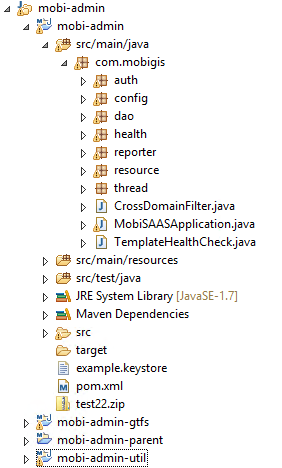
\includegraphics[width=6cm,heigth=6cm]{images/Package_explorer_MobiSAAS.PNG}
\caption{\label{Organisation_MobiAdmin}Organisation du module mobi-admin}
\end{figure} 

\\

\textbf{Hibernate :}

\begin{wrapfigure}{l}{3cm}
\centering

\includegraphics[width=3cm]{images/hibernate.png}
\end{wrapfigure}
\noindent Dans les langages objet, les données étant le plus souvent stockées dans des bases de données relationnelles ainsi l'utilisation d'un framework de mapping Objet/Relationnel est recommandé pour assurer la rapidité, l'évolutivité et la maintenabilité des développements. Hibernate, issu de la communauté Open Source, répond à ce besoin et connaît depuis quelques années un vif succès. Ce succès s'explique notamment par son architecture parfaitement adaptable à tout type de développements et le support de la majorité des bases de données du marché.\\

Afin de développer les classes pour la gestion des données clients (Uploads) du module «mobi-admin». J'ai mis en place une table « mobiuploads » sur le SGBD PostgreSQL (classes Upload.java, UploadDAO.java).
Grâce au framework Dropwizard, nous avons utilisé Hibernate comme ORM (Object Relationnal Mapping). J'ai pu ainsi manipuler mes objets (opérations CRUD) pour la création, la lecture, la mise à jour et la suppression des objets dans la base. 
Egalement, j'ai développé le chargement de ces données métiers (GTFS) dans le SGBD, j'ai mis en place le modèle de données et développer les classes avec les annotations Hibernate (@Entity, @Table, @JoinColumns,...). Ainsi, si le schéma n'existe pas il se génère automatiquement grâce à Hibernate. 
Toutes les requêtes sont écrites dans les classes java en HQL, langage propre à Hibernate grâce aux annotations @NamedQueries. \\


\textbf{Jackson :}

\begin{wrapfigure}{l}{3cm}
\centering
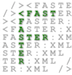
\includegraphics[width=3cm]{images/fxml_logo_Jackson.png}
\end{wrapfigure}
\noindent Jackson est une API JSON, elle est simple, bien documentée, et elle répond aux besoins suivants tels que :
\begin{itemize}
\item Capable de sérialiser et désérialiser des arbres JSON sans adhérence aux beans modèles.
\item Pouvant travailler directement sur des flux.
\item Capable de tenir une charge conséquente, donc stable et performante.
\item Avec le minimum possible de dépendances.
\end{itemize}

Afin que le service puisse renvoyer des réponses convenables et standards nous avons utilisé Jackson via Dropwizard \footnote{\url{http://www.mkyong.com/java/how-to-convert-java-object-to-from-json-jackson/}}. Grâce à la librairie Jackson nous pouvons transformer les \og beans \fg et convertir les propriétés java des objets en éléments Json, ainsi on renvoie par exemple le nom de l'upload, la date d'upload et surtout son status si l'opération c'est bien déroulée ou non (Fig. \ref{fig:Json1}).
\\
\begin{figure}[h]
	\centering
		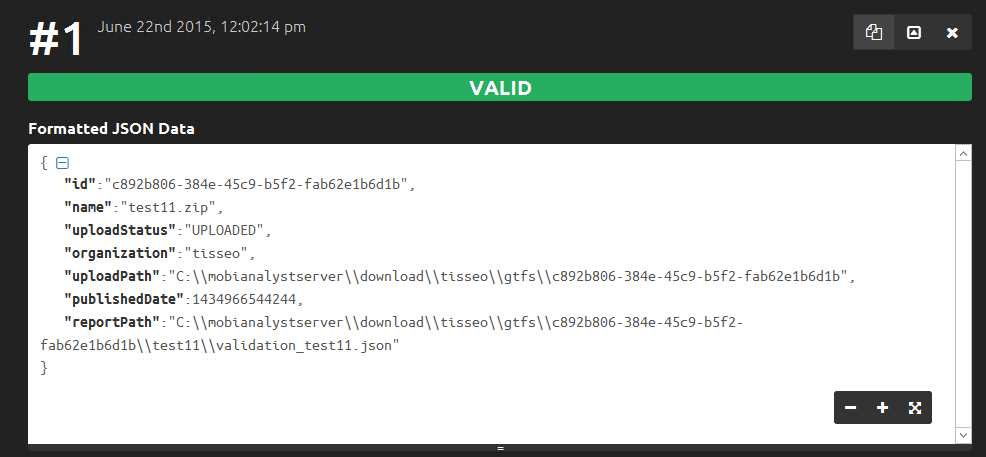
\includegraphics[width=0.8\textwidth]{images/JsonFormatter_serialization.PNG}
	\caption{Réponse Json renvoyée}
	\label{fig:Json1}
\end{figure}\\

De la même manière, chaque donnée GTFS, passe par un traitement métier de validation. Chaque Upload, possède donc une propriété appelée \og reportValidationPath \fg qui indique le chemin vers ce rapport de validation au format json. Ici, Jackson va permettre la production du rapport contenant les métadonnées et les anomalies pour chaque jeu de données GTFS (Fig. \ref{fig:Json2}).
\\
\begin{figure}[h]
	\centering
		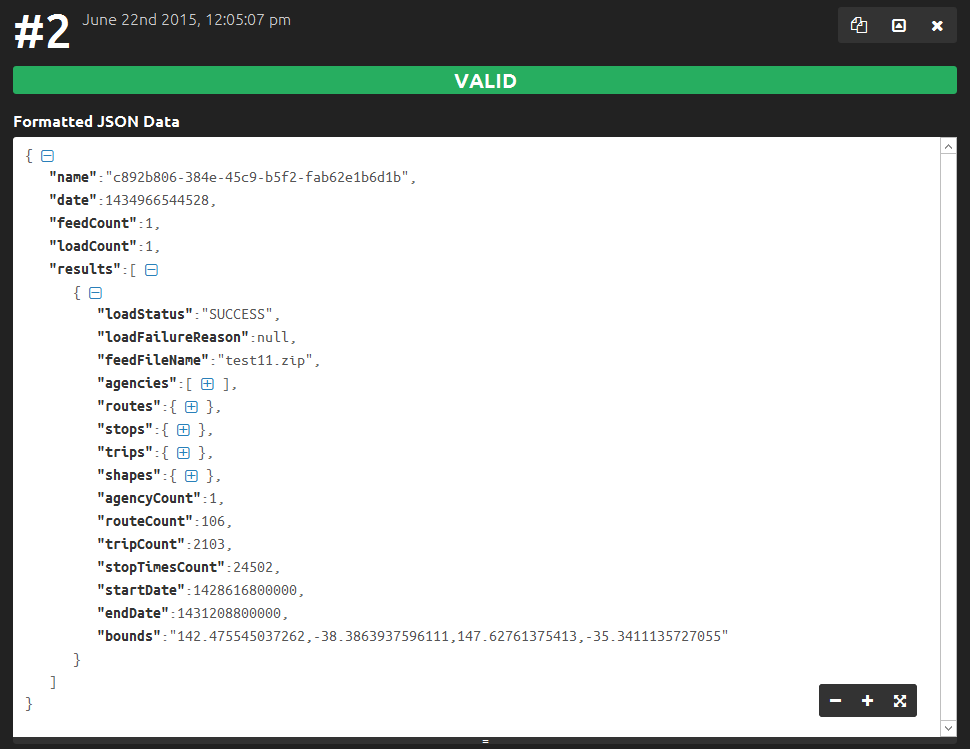
\includegraphics[width=0.8\textwidth]{images/JsonFormatter_serialization_Validation.PNG}
	\caption{Rapport Json de validation des données GTFS}
	\label{fig:Json2}
\end{figure}\\


\textbf{SLF4J et Logback :} 

\begin{wrapfigure}{l}{3cm}
\centering

\includegraphics[width=3cm]{images/slf4j-logo.jpg}

\includegraphics[width=3cm]{images/lblogo.jpg}
\end{wrapfigure}
\noindent SLF4J est une couche d'abstraction pour les API de journalisation Java. Le principe est à peu près similaire à celui de Jakarta Commons Logging. Les avantages de l'utilisation d'une telle couche d'abstraction permettent de s'abstraire de l'implémentation utilisée. Ainsi, il est possible de changer facilement d'implémentation de journalisation sans avoir à toucher la base de code. Au plus, la configuration de l'implémentation de journalisation doit être modifiée. Et enfin, dans le cas de la conception d'une librairie, cela permet de laisser à l'utilisateur de cette librairie le choix du système de journalisation.\\
Logback est un framework de logging. Logback est l'implémentation native de SLF4J, alors que son implémentation pour Log4J (ancêtre de Logback) est « wrappée ». De ce fait, il offre des fonctionnalités supplémentaires à Log4J.\\
Pour la gestion des traces (logs), j'ai donc pour chaque partie du code documenter et produit une trace intelligible à plusieurs niveaux d'informations : INFO, DEBUG, ERROR, etc... Encore une nouvelle fois , via Dropwizard l'utilisation d'un logger est facilité (cf. Extrait du log dans Annexe \ref{Annexe B}).

\textbf{JUnit :} 

\begin{wrapfigure}{l}{3cm}
\centering

\includegraphics[width=3cm]{images/junit-logo.png}
\end{wrapfigure}
\noindent JUnit est un framework de test unitaire por le langage Java, il s'intègre à l'IDE Eclipse. JUnit définit deux types de fichiers de tests. Les TestCase sont des classes contenant un certain nombre de méthodes de tests. Un TestCase sert généralement à tester le bon fonctionnement d'une classe. Une TestSuite permet d'exécuter un certain nombre de TestCase déjà définis. Pour notre cas, nous n'avons utilisé que des TestCase, pour tester de manière unitaire des fonctionnalités. Cet outil a été complémentaire des tests réaliser avec SoapUI.


\subsection{Réalisations}

J'ai tout d'abord commencé par découvrir Maven (cf. \ref{Maven}), les projets, les modules, le désormais célèbre fichier \textbf{POM}, etc...
Ensuite, je me suis documenté sur le code métier existant, et chercher des outils ou librairies de professionnels du domaine (cf. Outils métiers \ref{OBA}).
Enfin, après le \og Getting Started \fg de Dropwizard\footnote{\url{https://dropwizard.github.io/dropwizard/getting-started.html}}, une fois tout cela bien maîtrisé, j'ai pu commencé la conception et le développement de services web REST.\\

J'ai choisit de stocker les informations concernant ma partie de l'application dans une table PostgreSQL (Fig \ref{TablePostgres})\\
\begin{figure}[!h]
\centering
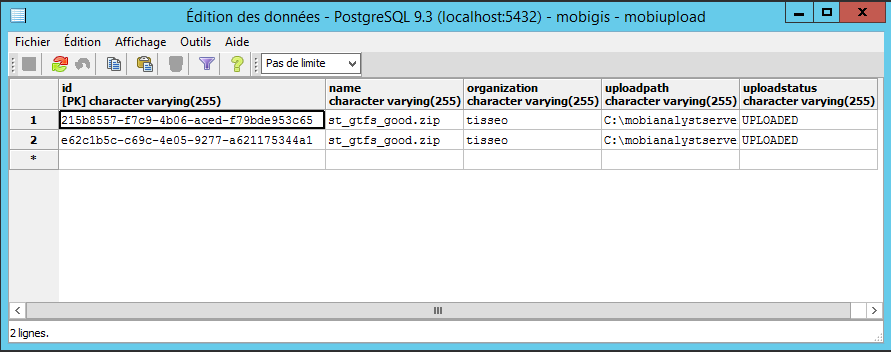
\includegraphics[width=14cm]{images/tablePostgres_mobiupload_small.png}
\caption{\label{TablePostgres}Table des uploads sur le SGBD PostgreSQL}
\end{figure} 

A chaque requête POST du client, je créé une instance d'objet Upload, les informations sont saisies dans la table de suivi, et je stocke les données envoyées sur le serveur. Pour chaque client ou utilisateur, pour chaque type de données, il y a un répertoire personnalisé, chaque upload est \og taggé \fg d'un identifiant unique \og UUID \fg.
Le code métier qui a été implémenté est pour le moment le test sur le type de données envoyées, la validation des données et la production d'un rapport d'un validation (JSON), enfin l'extraction (récursive) des données contenues dans l'archive (cf. Annexe \ref{Annexe B}).\\

A partir de ce service spécifique, dédié aux données GTFS, j'ai généralisé cette resource (FileResource.java) afin de permettre d'upload n'importe quel fichier sur le serveur, en réutilisant les mêmes méthodes, notamment celle de UploadDAO.java et la méthode \og métier \fg manageUpload().\\

Exemples de codes DAO :

exemple : UploadDAO

Exemples de codes Persistance /schéma de base de données : 

exemple : compositeKey
exemple : ManyToOne
exemple : com.mobigis.gtfs.model.Agency.java


Exemple de codes métiers :

exemple : GetBoundingBoxGtfs.java (geotools)

exemple : Jackson (ObjectMapper)


Exemple de test unitaires :

exemple : readWriteGTFS.java, completeTestGTFS.java
exemple : GtfsResourceTest.java

\paragraph{Tests}

Afin de tester les web services REST développés, j'ai utilisé fréquemment l'outil \textbf{SoapUI} (Fig. \ref{SoapUIGet}). Il permet de mettre en place une suite de tests qui peuvent être lancé d'une traite du côté client, permet de tester les services web en mode bouchon mais aussi d'effectuer des tests de charge. Il permet entre autre de fournir une hiérarchie des services web, de lister les différentes méthodes disponible, les paramètres attendus, de réaliser des requêtes et de récupérer les réponses … C'est l'un des meilleurs outils de test unitaires concernant les services web.\\

\begin{center}
\begin{figure}[h] \centering
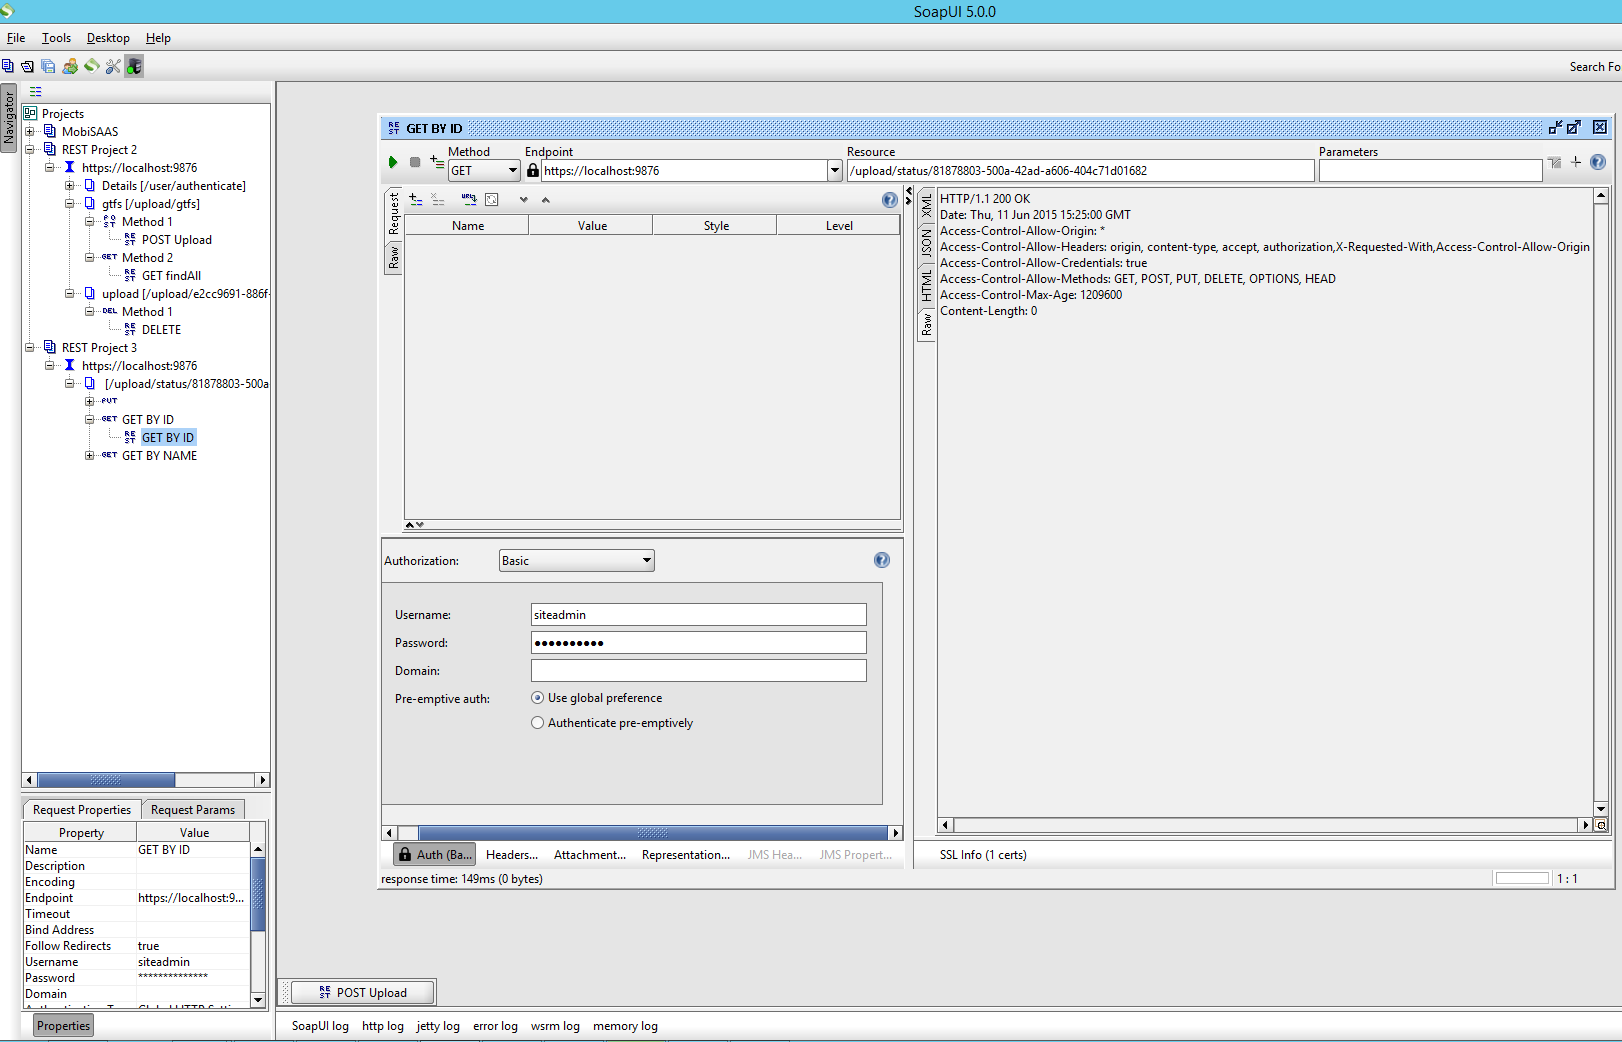
\includegraphics[width=16cm]{images/soapUI_getById_sansResponse_small.png}\\
\caption{\label{SoapUIGet} Interface et exemple de requête \og GET \fg SoapUI}
\end{figure}
\end{center}


\subsection{Perspectives}

L'idéal d'un programme développé dans un langage orienté objet, est la généricité, et la réutilisation d'un maximum de composants. Dans ce travail, l'objectif est clairement de produire un maximum de composant abstrait (classes et interfaces) et de méthodes réutilisables. Les perspectives du projet \og MobiSAAS \fg sont nombreuses : gérer une architecture distribuée, augmenter les fonctionnalités SAAS notamment les fonctionnalités de \og MobiAnalyst \fg, étendre le projet \og DataWizard \fg lui aussi mode SAAS.\\

J'ai donc \og maquetter l'application \fg et débuté le développement de ces composants abstraits (ex: Les ressources au sens DropWizard (Fig. \ref{UML1}). Grâce à cela on pourra donc \og uploader \fg plusieurs types de données et réutiliser la méthode manageUpload(). Egalement, sur ce même principe j'ai développé une classe abstraite afin de faire proposer la gestion des threads et tous mes services en hérite, cela limite la duplication de codes dans l'application.\\
\begin{figure}[!h]
\centering
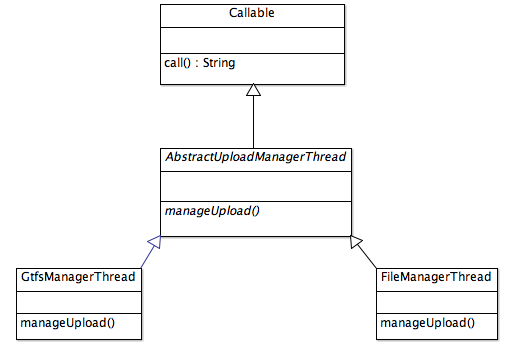
\includegraphics[width=14cm]{images/DiagrammeThread.png}
\caption{\label{UML1}Exemple d'abstraction et d'héritage de méthode}
\end{figure} 

J'ai commencé et non terminé un autre traitement de données spécifique au format GTFS. Une méthode de chargement des données dans la base de données Postgresql (méthode loadData()). J'utilise pour cela une librairie appelée OneBusAway\footnote{\url{http://onebusaway.org/developer-information/}} (OBA) spécialisée dans le transport. Ce traitement réalise une désérialization (lecture de fichiers csv) et une persistance des données via le framework Hibernate dans Postgresql. Ce qu'il reste à faire est de passer la méthode en resource.





\pagebreak

\section{DataWizard}\label{DataWizard}

\subsection{Cahier des charges, présentation de l'application}

Le projet \og DataWizard \fg, ensemble de scripts Python et SQL est une application dont le but est d'ingérer des données de transports, et de voirie dans une base de données spatiales (\textbf{PostGIS}\ref{Postgis}) afin de produire en sortie un réseau de transport (Network Dataset ou NDS).\\


\subsection{Eléments de spécifications fonctionnelles}

Le DataWizard permet de se lancer par étapes. Il y a 10 étapes successives, dont une étape préliminaire appelée étape 0, et une indépendante : l'étape 10.
\begin{itemize}
\item STEP 0 : Nettoyage et préparation de la base de données
\item STEP 1 : Import des données transport en commun et conversion vers le schéma mobianalyst
\item STEP 2 : Import des données de voirie
\item STEP 3 : Import des données métro et conversion vers le schéma mobianalyst
\item STEP 4 : Génération des données vitesses moyennes et horaires et connexion des réseaux de transport en commun et voirie
\item STEP 5 : Calcul des horaires et des vitesses moyennes
\item STEP 6 : Export des données vers des fichiers Shapefile (.shp)
\item STEP 7 : Import des données dans la Géodatabase de sortie et changement du système de projection si nécessaire
\item STEP 8 : Extraction des différents modes, génération du fichier xml servant à construire le réseau et de MobiNetwork.xml
\item STEP 9 : Construction et compilation du réseau
\item STEP 10 : Production de métadonnées pour le réseau
\end{itemize}

Afin de fournir, un réseau conforme aux attentes du logiciel MobiAnalyst \og version 3.0 \fg et des experts en analyse de réseaux de transports, l'équipe me fournit une spécification de métadonnées à extraire des données en entrée du DataWizard (Fig. \ref{DW_Metadata}).\\

\begin{figure}[!h]
\centering
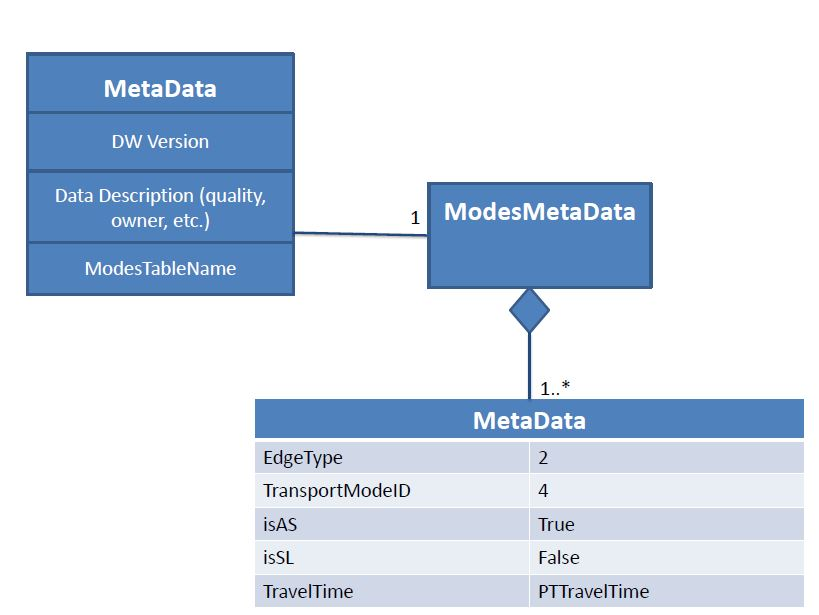
\includegraphics[width=12cm]{images/DW_specMetadata.JPG}
\caption{\label{DW_Metadata}Métadonnées de réseau de transports v3.0}
\end{figure} 

\subsection{Eléments de spécifications techniques}

J'intègre tout d'abord le projet en tant qu'utilisateur, j'exploite des données et produits des réseaux de transport en commun (TC) (Bordeaux, Champagne-Ardennes, Montreal, Melbourne,etc...) Ensuite, petit à petit je suis le plan de charge issu du projet Redmine et corrige des bugs, et anomalies.\\

Mon premier travail a été de développer l'étape 10 (STEP 10 : Export Metadata Tables) de l'exécution du DataWizard. Pour cela j'ai du extraire le nombre de mode de transports en commun (variable selon chaque projet), leur code (variable selon chaque projet) et enfin extraire des listes de constantes pour documenter le réseau produit par le DataWizard.\\

Exemple ?\\

Un autre travail réalisé est le développement qui permet la gestion du système de projection des données géographiques pour les calculs du DataWizard. Cette modification impacte quasiment la totalité des requêtes SQL dites spatiales de l'application, et permet des résultats (calculs de distances) plus réalistes (par exemple pour Melbourne, Australie située dans l'hémisphère Sud).\\


\subsection{Réalisations}

Les principales difficultés concernent les données. Ces données sont complexes, les données GTFS ou les données de voirie (données Here (anciennement Navteq) ou OpenStreetMap\footnote{\url{http://openstreetmap.fr/}}). La base de données \og DataWizard \fg possède ainsi de nombreux schémas, et les requêtes SQL sont parfois très complexes mêlant fonctions, et requêtes géographiques.\\

Les résultats obtenus sont la production de nombreux réseaux en version 3.0 (avec les métadonnées) pour nos analystes, et pour les projets nécessitant des réseaux récents (Moveazy, Mobilyse, etc...). Et une version de l'application qui je l'espère est plus stable.\\

Exemple de code pour produire une table de métadonnées (Fig. \ref{CodeMetadata}) :
\\
\begin{figure}[h]
	\centering
		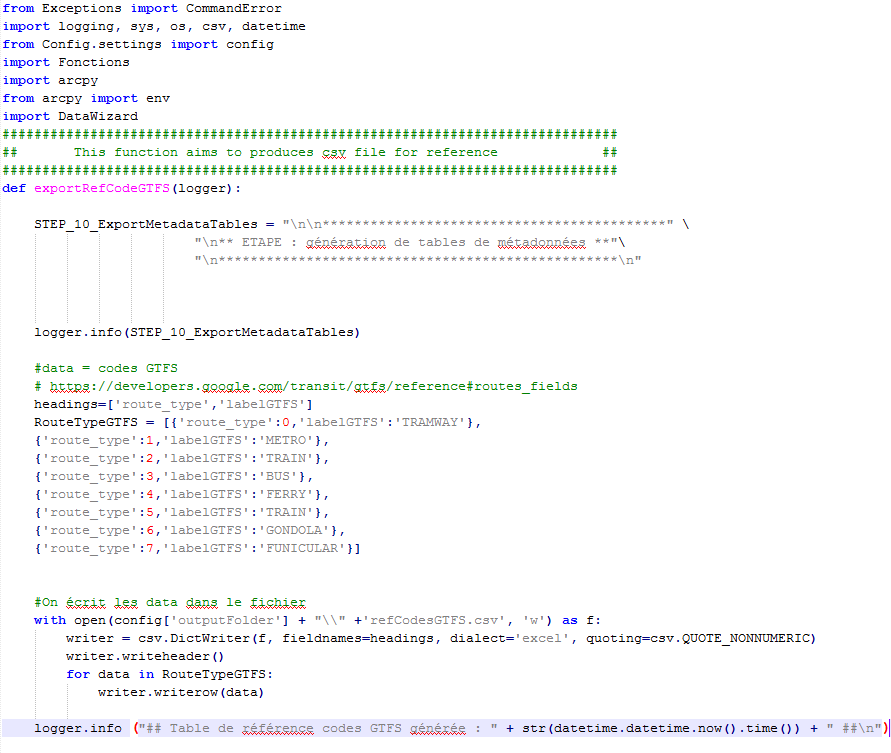
\includegraphics[width=0.8\textwidth]{images/DW_Fonction_Python.PNG}
	\caption{Fonction Python pour exporter des métadonnées}
	\label{CodeMetadata}
\end{figure}\\

Dans ce projet, j'ai également développé des fonctions utilitaires : BOMConverter.py, searchAndReplaceFiles.py, etc... Ces méthodes permettent notamment de formater les données avant leur import dans la base de données. Cela peut certainement éviter les mauvaises surprises d'encodage ou de caractères spéciaux fréquemment rencontrés lors de l'exploitation de données GTFS.\\




Exemples langages de bases de données :

exemple requête PostGIS




\subsection{Perspectives}

La liste des évolutions sur le projet Redmine est longue, il y a en effet énormément de perspectives pour le projet... Tout d'abord permettre l'import de plusieurs formats de données, comme l'import de données \og Shapefile \fg qui n'est pas encore terminé, mais aussi de données de transports en commun \og Trident \fg... Augmenter encore la capacité de l'outil à rendre ses étapes indépendantes, nettoyer les fonctions obsolètes, revoir l'algorithme de certaines méthodes,...
Les tests que j'ai pu faire démontre que c'est une application gourmande en RAM, et que les accès disques (lecture/écriture) sont vite à saturation. D'une manière générale les besoins pour l'application sont d'optimiser les étapes, et développer des routines de simplification de données afin par exemple de ne retenir que les données nécessaires au traitement au lieu de charger toutes les données en amont,... \\


\section{Crislab}\label{Divers}

\subsection{Présentation} 

Ce projet est dédié à la Cartographie des RISques de LABoratoire. Il consiste en une application web, proposant une interface cartographique des bâtiments afin de permettre la gestion des marqueurs et relevés de zones à risques. La vocation de l'application est un site intranet. Durant mon stage, j'ai eu de nombreux échanges avec le client afin de résoudre des bugs de l'application. J'ai donc participé au débugage et à la production de nouveaux livrables (.war).\\

Le projet est très complet, et présente une architecture assez typique d'une application web (cf. Annexe \ref{Annexe C}). Ainsi, l'interface Homme-Machine (IHM) est codée en Javascript, il y a de nombreux formulaires d'affichage ou de saisie dans des fichiers JSP  (Java Server Pages), la partie cartographique est encore une fois produite par un serveur ArcGIS dédié. Le serveur d'applications est un serveur Tomcat 6, adossé sur un SGBD Oracle 10g. Toute la persistance est gérée via le framework Hibernate.\\

\begin{figure}[h]
	\centering
		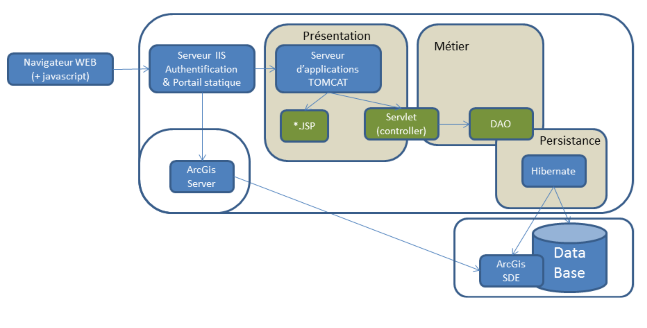
\includegraphics[width=0.8\textwidth]{images/Architecture_Crislab.PNG}
	\caption{Architecture globale de l'application Crislab}
	\label{fig:architecture}
\end{figure}\\


\subsection{Réalisations}

J'ai donc \og administré \fg le projet sous Eclipse avec Maven, j'ai lancé l'application sur un serveur Tomcat, créer différents profils de configuration (développement, tests, production) avec des propriétés de connexion différentes à chaque profil). J'ai testé l'application avec le navigateur \og client \fg Internet Explorer 11. Ce projet m'a permis de mettre en application mes connaissances client-serveur, sur toute la partie présentation d'une application web depuis l'affichage des JSP jusqu'aux actions déclenchées (couche service) interceptées par les contrôleur.\\

Le debug a surtout consisté à reproduire les bugs de l'application en production. Du coup, j'ai du importer le schéma de la base de données (Oracle) des clients, tester les requêtes de mon service sur leurs données. J'ai essentiellement passé mon temps à refaire les requêtes, et notamment traduire le HQL (langage de requête Hibernate) en SQL (langage de requête \og standard \fg). Par exemple, le premier bug était du à une mauvaise initialisation d'une variable (fixée à 1 au lieu de 2)... Un deuxième bug venait lui d'une mauvaise manipulation de l'opérateur qui avait provoquer la création d'un doublon dans la base... (chose impossible à réaliser via l'interface cliente (IHM)).\\


\chapter{Discussion}






\chapter{Glossaire et définitions}
\label{Glossaire}

\textbf{API} : En informatique, une interface de programmation (souvent désignée par le terme API pour Application Programming Interface) est un ensemble normalisé de classes, de méthodes ou de fonctions qui sert de façade par laquelle un logiciel offre des services à d'autres logiciels. Elle est offerte par une bibliothèque logicielle ou un service web, le plus souvent accompagnée d'une description qui spécifie comment des programmes consommateurs peuvent se servir des fonctionnalités du programme fournisseur.

Des logiciels tels que les systèmes d'exploitation, les systèmes de gestion de base de données, les langages de programmation, ou les serveurs d'applications comportent une interface de programmation\footnote{\url{http://fr.wikipedia.org/wiki/Interface_de_programmation}}.\\

\textbf{Eclipse} : L'environnement de programmation (IDE) en langage Java le plus connu est le projet "Eclipse" de la fondation Eclipse. Ce logiciel simplifie la programmation grâce à un certain nombre de raccourcis et notamment grâce à la possibilité d'intégrer de nombreuses extensions. Au fur et à mesure de l'avancement du code, Eclipse compile automatiquement le code et signale les problèmes qu'il détecte.\\

\textbf{Géomatique} : La géomatique est la combinaison syntaxique de deux mots : Géographie et Informatique.
Le mot géomatique a été déterminé pour regrouper de façon cohérente l’ensemble des connaissances et technologies nécessaires à la production et au traitement des données numériques décrivant le territoire, ses ressources ou tout autre objet ou phénomène ayant une position géographique.
La géomatique est un domaine qui fait appel aux sciences, aux technologies de mesure de la terre ainsi qu’aux technologies de l’information pour faciliter l’acquisition, le traitement et la diffusion des données sur le territoire (aussi appelées "données spatiales ", "données géospatiales" ou " données géographiques").
La géomatique est étroitement liée à l’information géographique qui est la représentation d’un objet ou d’un phénomène localisé dans l’espace.
Ainsi, la géomatique regroupe l’ensemble des outils et méthodes permettant de représenter, d’analyser et d’intégrer des données géographiques
\footnote{\url{http://www.sig-geomatique.fr/sig-geomatique.html}}.\\

\textbf{Java} : Java est un langage orienté objet, c'est-à-dire que le programme est vu comme un ensemble d'entités (de classes). Au cours de l'exécution du programme, les entités collaborent entre elles pour arriver à un but commun.\\

\textbf{POM} : Chaque projet ou sous-projet est configuré par un POM "Project Object Model" qui contient les informations nécessaires à Maven pour traiter le projet (nom du projet, numéro de version, dépendances vers d'autres projets, bibliothèques nécessaires à la compilation, noms des contributeurs etc.). Ce POM se matérialise par un fichier pom.xml à la racine du projet. Cette approche permet l'héritage des propriétés du projet parent. Si une propriété est redéfinie dans le POM du projet, elle recouvre celle qui est définie dans le projet parent. Ceci introduit le concept de réutilisation de configuration. Le fichier pom du projet principal est nommé pom parent. Il contient une description détaillée de votre projet, avec en particulier des informations concernant le versionnage et la gestion des configurations, les dépendances, les ressources de l'application, les tests, les membres de l'équipe, la structure et bien plus.\\

\textbf{PostgreSQL} : PostgreSQL est un système de gestion de bases de données relationnelles objet (Manuel PostgreSQL). PostgreSQL est un outil Open Source et disponible gratuitement, compatible avec les systèmes d'opérations les plus connus (Linux, Unix (Mac OSX, Solaris etc.) et Windows). PostgreSQL propose des interfaces de programmations pour des langages de programmation comme Java, C++, Python etc.
Le développement de PostgreSQL a débuté en 1986 (appelé à l'époque Postgres). En 1995, les développeurs ajoutent un interpréteur de langage SQL à l'outil. A partir de 1996, l'outil s'appelle PostgreSQL afin de souligner le lien entre Postgres et le langage SQL. PostgreSQL peut être facilement étendu par l'utilisateur en ajoutant de nouvelles fonctions, de nouveaux opérateurs ou même de nouveaux langages de procédure.\\

\textbf{PostGIS} : PostGIS est une extension du système de gestion de base de données PostgreSQL qui permet de stocker des données (objets) géographiques dans la base de données. Cette extension permet d'utiliser une base de données PostgreSQL comme une base de données dans n'importe quel projet SIG. PostGIS est compatible avec de nombreux autres outils SIG comme par exemple QGIS, Mapserver, etc...\\

\textbf{REST} : REST "Representational State Transfer" (REST) ​​est un style d'architecture logicielle comprenant des lignes directrices et des meilleures pratiques pour la création de services Web évolutifs. REST est un ensemble coordonné de contraintes appliqué à la conception de composants dans un système hypermédia distribué qui peut conduire à une architecture plus performante et maintenable.

REST a gagné sa réputation à travers le web comme une alternative plus simple à SOAP et des services basés sur un WSDL. Les systèmes "RESTful" peuvent généralement, mais pas toujours, communiquer avec les verbes du protocole HTTP (GET, POST, PUT, DELETE, etc.) utilisés par les navigateurs Web pour récupérer des pages Web et envoyer des données à des serveurs distants.\\


\textbf{SAAS} : SAAS "Software as a Service" Le logiciel en tant que service est un modèle d'exploitation commerciale des logiciels dans lequel ceux-ci sont installés sur des serveurs distants plutôt que sur la machine de l'utilisateur. Les clients ne paient pas de licence d'utilisation pour une version, mais utilisent généralement gratuitement le service en ligne ou payent un abonnement récurrent\footnote{\url{http://fr.wikipedia.org/wiki/Logiciel_en_tant_que_service}}.\\

\textbf{SoapUI} : SoapUI est outil graphique qui permet de tester des services web basés sur diverses technologies. Il est disponible en deux versions : une version gratuite et open source et seconde version payante. Il est également disponible sous forme de plugin pour les IDE Netbeans, IntelliJ IDEA et Eclipse. SoapUI est développé entièrement en Java et utilise Java Swing pour son GUI, il fonctionne donc sur la plupart des systèmes d'exploitation et en plus il est disponible sous licence GNU.
L'outil gère respectivement les services web basés sur les technologies telles que le HTTP (S), HTML, SOAP (WSDL), REST, AMF, JDBC et JMS.\\

\textbf{SVN} : SVN ou Subversion est un système de gestion de version, conçu pour remplacer CVS. Concrètement, ce système permet aux membres d’une équipe de développeur de modifier le code du projet quasiment en même temps. Le projet est en effet enregistré sur un serveur SVN et à tout moment, le développeur peut mettre à jour une classe avant de faire des modifications pour bénéficier de la dernière version et a la possibilité de comparer deux versions d'un même fichier.\\

\textbf{WS} : Acronyme de "Web Service" ou Service Web. Un WS est un programme informatique de la famille des technologies web permettant la communication et l'échange de données entre applications et systèmes hétérogènes dans des environnements distribués. Il s'agit donc d'un ensemble de fonctionnalités exposées sur internet ou sur un intranet, par et pour des applications ou machines, sans intervention humaine, de manière synchrone ou asynchrone. Actuellement, le protocole de transport est essentiellement HTTP(S)\footnote{\url{http://fr.wikipedia.org/wiki/Service_web}}. \\



\chapter{Annexes}
\label{Annexes}

\section{Apache Maven}\label{Annexe A}\\

\textbf{Apache Maven} est un outil pour la gestion et l'automatisation de production des projets logiciels Java en général et Java EE en particulier. L'objectif recherché est comparable au système Make sous Unix : produire un logiciel à partir de ses sources, en optimisant les tâches réalisées à cette fin et en garantissant le bon ordre de fabrication.\\
Il est semblable à l'outil Ant, mais fournit des moyens de configuration plus simples, eux aussi basés sur le format XML. Maven est géré par l'organisation Apache Software Foundation. Précédemment Maven était une branche de l'organisation Jakarta Project.\\
Maven utilise un paradigme connu sous le nom de Project Object Model (POM) afin de décrire un projet logiciel, ses dépendances avec des modules externes et l'ordre à suivre pour sa production. Il est livré avec un grand nombre de tâches pré-définies, comme la compilation de code Java ou encore sa modularisation.\\
Un élément clé et relativement spécifique de Maven est son aptitude à fonctionner en réseau. Une des motivations historiques de cet outil est de fournir un moyen de synchroniser des projets indépendants : publication standardisée d'information, distribution automatique de modules « jar ». Ainsi en version de base, Maven peut dynamiquement télécharger du matériel sur des dépôts logiciels connus. Il propose ainsi la synchronisation transparente de modules nécessaires.\\

\pagebreak

\section{DropWizard}\label{Annexe B}\\

\textbf{Dropwizard} est un framework Java léger adapté au développement rapide de microservices REST et ne nécessitant pas de serveur d’application comme environnement d’exécution. \\
Cela dit, au delà du framework, c’est surtout un assemblage habile de composants spécialisés parmi les meilleurs de l’écosystème Java :
\begin{itemize}
\item \textbf{Jetty}, un serveur HTTP et un moteur de servlet compacts et très performants 
\item \textbf{Jersey}, l’implémentation de référence de la spécification JAX-RS (web services REST) 
\item \textbf{Jackson}, une librairie de sérialisation/dé-sérialisation JSON 
\item \textbf{Hibernate Validator}, l’implémentation de référence de l’API Bean Validation (JSR 303) 
\item \textbf{SLF4J} et \textbf{Logback} pour la gestion des traces 
\item \textbf{Metrics} pour le monitoring 
\item \textbf{jDBI} pour l’interfaçage rapide à une base de données relationnelle. Cette librairie est de bien plus bas niveau que JPA ou Hibernate et présente peu d’abstraction ce qui rend sa prise en main aisée \\
\end{itemize}

Packagée sous la forme d’un jar autonome contenant toutes ses dépendances, l’unité de déploiement n’a pas besoin de serveur d’application pour être exécutée (le conteneur Jetty est embarqué dans le jar). Avec ses 10 Mo tout au plus (dépendances comprises) l’empreinte mémoire d’une application Dropwizard est donc incomparablement plus faible qu’un Web Service SOAP déployé dans un serveur d’application Java EE (jusqu’à plusieurs centaines de Mo).
En conséquences, le temps de démarrage d’une application Dropwizard est de quelques secondes quand il faut parfois plusieurs minutes pour un serveur d’application.\\

\pagebreak


\section{Redmine}\label{Annexe C}

Redmine est considéré comme l’un des outils de gestion de projets collaboratifs Open Source parmi les plus aboutis. Il recouvre un ensemble de fonctionnalités dont un aperçu est donné ci-dessous, comme la gestion multi-projets, la gestion des demandes d’évolution et des bugs, la gestion et l’indexation des documentations techniques, mais aussi la gestion des droits et des profils des différents intervenants. Il propose aussi une console de suivi de l’état d’avancement des projets, des tâches, des recettes… sous forme de diagramme de Gantt.\\

Redmine est une forge logicielle sous licence GPL. Ses principaux concurrents se nomment Trac, Retrospectiva, Django Projector ou encore InDefero. Notons que Jira ne trouve pas sa place ici, bien qu’il soit le concurrent le plus sérieux de Redmine, parce que Jira est sous Dual licence (l’utilisation commerciale nécessite une licence payante non-Open Source).\\

Redmine offre un ensemble de fonctionnalités comme par exemples :

\begin{itemsize}
\item Prise en charge de plusieurs projets
\item Contrôle d’accès avec un modèle flexible de rôles
\item Gestion avancée des tickets
\item Diagramme de Gantt et calendrier
\item Publication de news, documents et gestionnaire de fichiers
\item Notifications par emails et flux ATOM
\item Wiki et forums par projet
\item Outil de suivi du temps
\item Champs personnalisables pour les tickets, suivi de temps, projets et utilisateurs
\item Intégration avec plusieurs SCM : SVN, CVS, Git, Mercurial, Bazaar et Darcs
\item Une communauté active et un ensemble d’outils connexes
\end{itemsize}\\

Plus de détails est disponible sur le wiki du projet : \url{http://www.redmine.org/projects/redmine/wiki}.

\pagebreak

\section{Extraits de codes}\label{Annexe D}\\

\textbf{Instanciation d'un objet upload}\\
\begin{lstlisting}
	// Instanciation
	Upload up = new Upload();
	up.setId(CreateUUID.randomUUID().toString());
	up.setOrganization(user.getOrganization());
	up.setName(fileDetails.getFileName());
\end{lstlisting} \\

\textbf{La classe Upload.java associée}\\

\begin{lstlisting}
	// Empty constructor
	public Upload (){
	}

    // Constructor
    public Upload(String id, String name, String uploadStatus, String organization, String uploadPath){
        super();
        this.id=id;
        this.name = name;
        this.uploadStatus = uploadStatus;
        this.organization = organization;
        this.uploadPath = uploadPath;
    }
    
    // Getters & Setters
    public String getId() {
        return id;
    }

    public void setId(String id) {
        this.id = id;
    }
    
    public String getName() {
        return name;
    }

    public void setName(String name) {
        this.name = name;
    }

    public String getUploadStatus() {
        return uploadStatus;
    }

    public void setUploadStatus(String uploadStatus) {
        this.uploadStatus = uploadStatus;
    }

    public String getOrganization() {
        return organization;
    }

    public void setOrganization(String organization) {
        this.organization = organization;
    }

    public String getUploadPath() {
        return uploadPath;
    }

    public void setUploadPath(String uploadPath) {
        this.uploadPath = uploadPath;
    }
	// suite des Getters & Setters
\end{lstlisting} \\

\textbf{Classe UploadDAO.java}\\

\begin{lstlisting}
	// Create 
    public String create(Upload up)
    {
        System.out.println("Upload instance created : "+up.getId()+" | "+up.getName()+" | "+up.getUploadStatus()+" | "+up.getOrganization()+" | "+up.getUploadPath());
        return persist(up).getId();
    }

    // Read one
    public Upload findByID(String id)
    {
        //return get(id);
        Query query = namedQuery("com.mobigis.dao.Upload.findByID");
        query.setParameter("id", id);
        List<Upload> res = list(query);
        if(res != null && res.size()>0)
        {
            return res.get(0);
        }
        return null;
    }
\end{lstlisting} \\


\textbf{Extrait du log Eclipse}\\

\begin{lstlisting}
INFO  [2015-06-11 15:31:52,883] com.mobigis.thread.AbstractUploadManagerThread: GTFS validation JSON report done !
file unzip : agency.txt
file unzip : calendar.txt
file unzip : calendar_dates.txt
file unzip : fare_attributes.txt
file unzip : fare_rules.txt
file unzip : frequencies.txt
file unzip : routes.txt
file unzip : shapes.txt
file unzip : stop_times.txt
file unzip : stops.txt
file unzip : trips.txt
Extract Done
Clean directory Done
upload status = UPLOADED
INFO  [2015-06-11 15:31:52,920] com.mobigis.thread.AbstractUploadManagerThread: Process upload to Location = C:\mobianalystserver\download\tisseo\gtfs\215b8557-f7c9-4b06-aced-f79bde953c65
INFO  [2015-06-11 15:31:52,920] com.mobigis.thread.AbstractUploadManagerThread: Upload file done ! Id = 215b8557-f7c9-4b06-aced-f79bde953c65 | Status = UPLOADED
C:\mobianalystserver\download\tisseo\gtfs\215b8557-f7c9-4b06-aced-f79bde953c65
INFO  [2015-06-11 15:31:52,965] org.hibernate.engine.internal.StatisticalLoggingSessionEventListener: Session Metrics {
    36877 nanoseconds spent acquiring 1 JDBC connections;
    0 nanoseconds spent releasing 0 JDBC connections;
    358836 nanoseconds spent preparing 4 JDBC statements;
    6286839 nanoseconds spent executing 4 JDBC statements;
    0 nanoseconds spent executing 0 JDBC batches;
    0 nanoseconds spent performing 0 L2C puts;
    0 nanoseconds spent performing 0 L2C hits;
    0 nanoseconds spent performing 0 L2C misses;
    24185654 nanoseconds spent executing 1 flushes (flushing a total of 2 entities and 2 collections);
    42650 nanoseconds spent executing 1 partial-flushes (flushing a total of 0 entities and 0 collections)
}
127.0.0.1 - - [11/Jun/2015:15:31:50 +0000] "POST /upload/gtfs HTTP/1.1" 200 61 "-" "Apache-HttpClient/4.1.1 (java 1.5)" 2254
\end{lstlisting} 


\pagebreak

\section{Structure d'une application Web}\label{Annexe E}\\


\begin{figure}[!h]
\centering
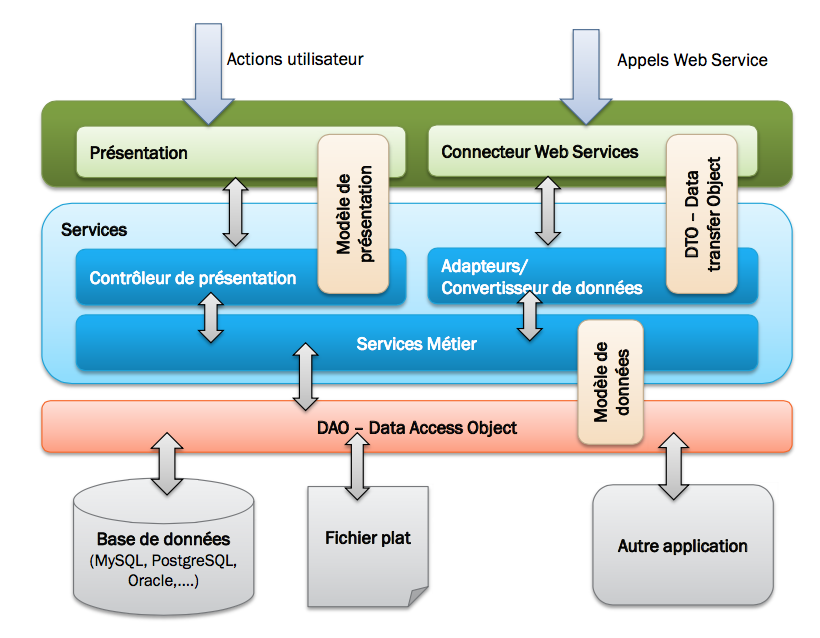
\includegraphics[width=\textwidth]{images/WebAppArchitecture.png}
\caption{\label{WebAppArchitecture}Structure d'une application Web}
\end{figure} 



\chapter*{Webographie}
\label{Bibliographie}


\textbf{Sites sur les données/outils "métiers" :}\label{OBA}\\


\url{https://developers.google.com/transit/gtfs/examples/gtfs-feed}\\

\url{https://developers.google.com/transit/gtfs/}\\

\url{https://github.com/google/transitfeed/wiki/FeedValidator}\\

\url{http://onebusaway.org/developer-information/}\\

\url{https://github.com/OneBusAway/onebusaway/wiki/Importing-source-code-into-Eclipse}\\


\textbf{Sites sur les frameworks et outils utilisés :}\\


\url{http://www.objis.com/formation-java/tutoriel-formation-maven-2.html}\\

\url{http://mvnrepository.com/}\\

\url{https://github.com/bucharest-jug/dropwizard-todo}\\

\url{http://docs.jboss.org/hibernate/orm/4.3/manual/en-US/html/}\\

\url{http://www.tutorialspoint.com/hibernate/}\\

\url{http://blog.xebia.fr/2011/11/14/rest-java-serveur/}\\


Et pour finir, un grand merci à \url{http://www.mkyong.com/}, tout simplement.

\nocite{*}
\bibliographystyle{apalike-fr} % Le style est mis entre crochets.
%\bibliography{RapportBiblio}

%\section{Principes généraux}

testt



\end{document}